\subsection{Model Evaluation and Interpretation}

\subsubsection{Test Set Evaluation}

The final selected model is the pretrained ResNet-34 baseline without additional attention modules, trained using the hyperparameters obtained from the hyperparameter analysis stage. The model achieves a test accuracy of 92.53\%, compared with a validation accuracy of 95.38\%. This result indicates a moderate generalization gap between the validation and test sets while still maintaining strong overall performance.

\subsubsection{Confusion Matrix Analysis}

Figure~\ref{fig:confusion_matrix} presents the confusion matrix on the test set. Most classes are classified accurately, while several visually similar breeds exhibit noticeable confusion.

\begin{figure}[htbp]
    \centering
    
\includegraphics[width=0.92\textwidth]{figures/task1/confusion_matrix.png}
    \caption{Confusion matrix of the best ResNet-34 model on the test set.}
    \label{fig:confusion_matrix}
\end{figure}

The most frequent confusion pairs include:
\begin{itemize}
    \item American Pit Bull Terrier $\rightarrow$ Staffordshire Bull Terrier (22 samples),
    \item American Pit Bull Terrier $\rightarrow$ American Bulldog (14 samples),
    \item Staffordshire Bull Terrier $\rightarrow$ American Pit Bull Terrier (13 samples),
    \item Ragdoll $\rightarrow$ Birman (13 samples),
    \item Egyptian Mau $\rightarrow$ Bengal (10 samples).
\end{itemize}

These errors mainly occur between breeds sharing highly similar facial structures, fur patterns, or body shapes. The confusion matrix therefore suggests that the remaining classification difficulty is largely caused by small inter-class visual differences rather than severe optimization failure.

\subsubsection{Error Case Analysis}

Representative failure cases are shown in Figure~\ref{fig:error_examples}.

\begin{figure}[htbp]
    \centering
    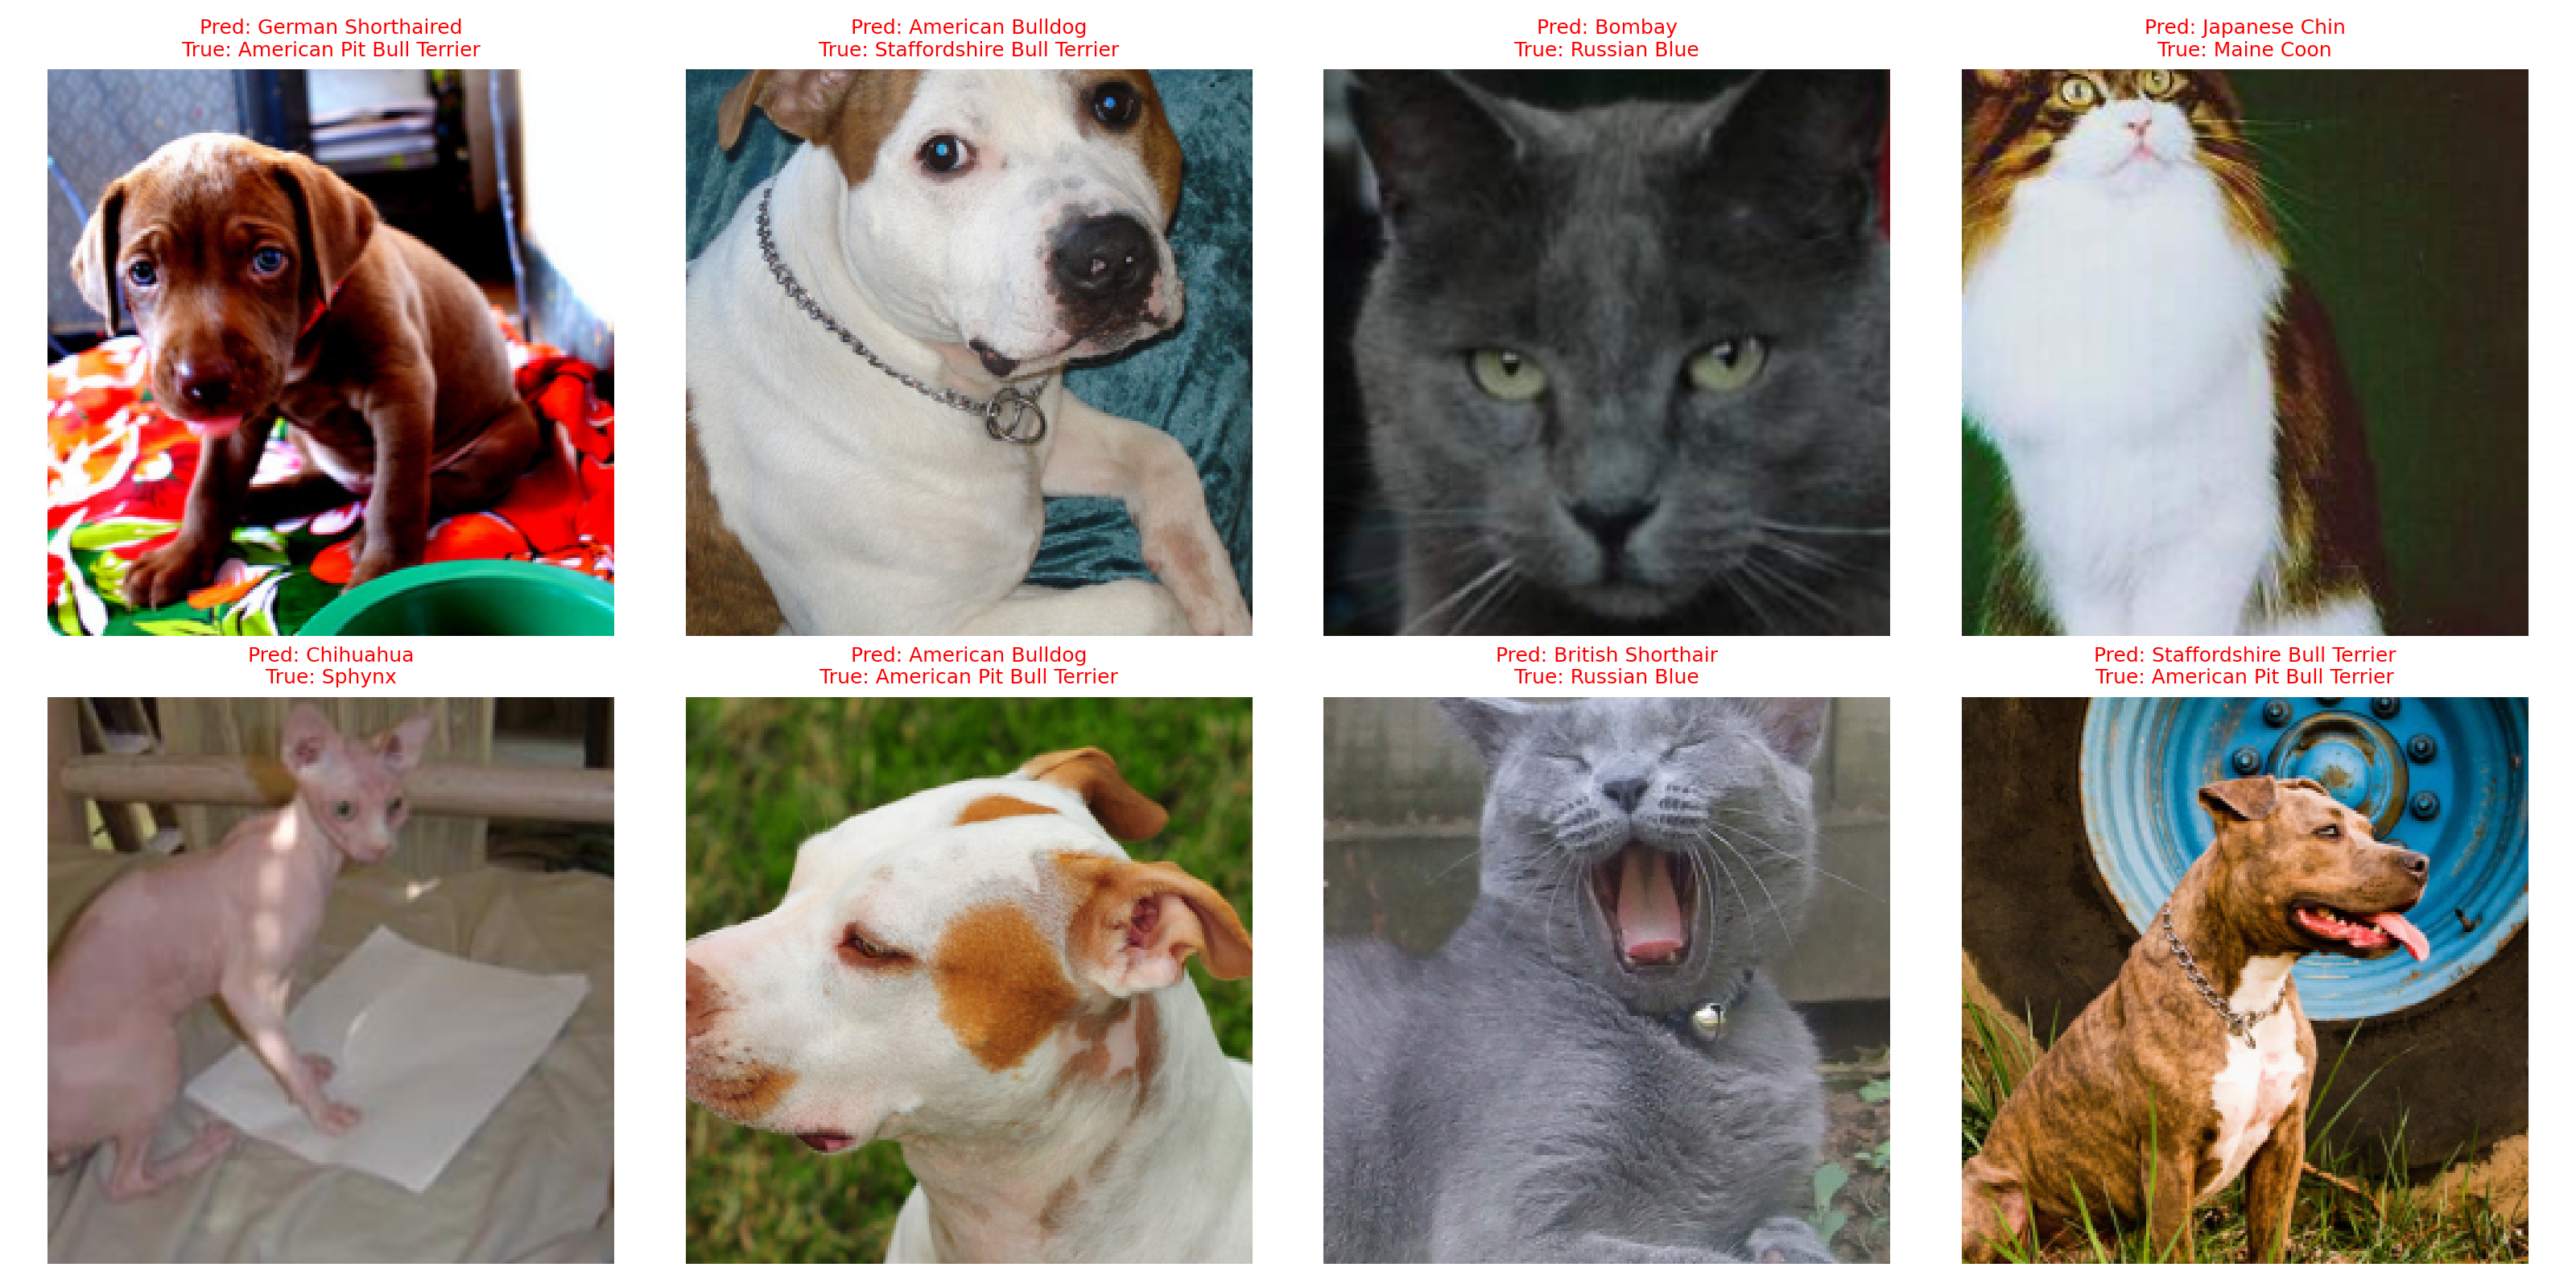
\includegraphics[width=0.9\textwidth]{figures/task1/error_example.png}
    \caption{Representative misclassified examples from the test set.}
    \label{fig:error_examples}
\end{figure}

Several factors may contribute to these errors. First, due to the fixed input resolution requirement, center cropping may remove important semantic cues such as ears, noses, or partial facial regions. Second, certain breeds are inherently difficult to distinguish because of strong visual similarity. Third, unusual lighting conditions may introduce distribution shifts not sufficiently covered during training. For example, strong local illumination appearing only on part of the animal body may alter texture statistics learned by the network. Finally, uncommon poses or expressions, such as yawning or heavily rotated heads, may also reduce prediction confidence.

\subsubsection{Feature Visualization with DeepDream}

To further investigate the visual features learned by the network, DeepDream visualizations are generated for several representative classes. Figure~\ref{fig:deepdream_results} compares representative input images with the DeepDream visualizations of their corresponding classes.

\begin{figure}[H]
    \centering
    
    \begin{minipage}{0.2\textwidth}
        \centering
        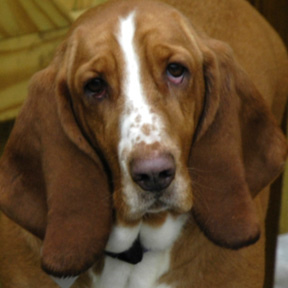
\includegraphics[width=\textwidth]{figures/task1/basset_hound_151.jpg}
    \end{minipage}
    \begin{minipage}{0.28\textwidth}
        \centering
        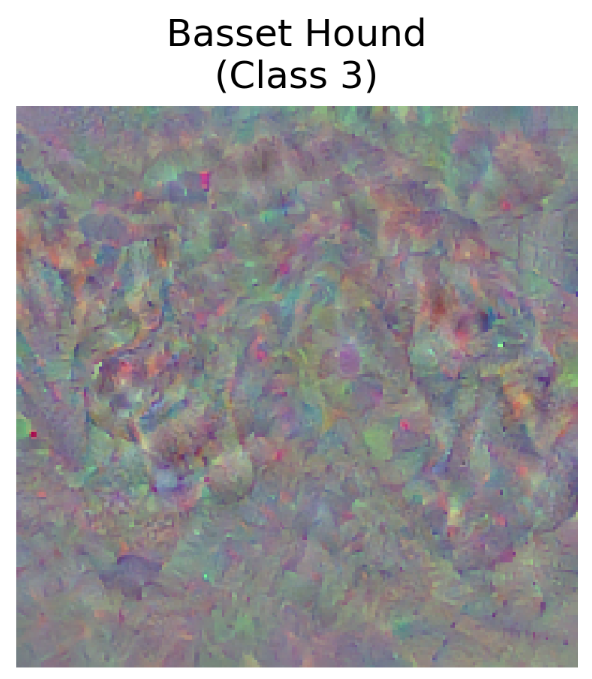
\includegraphics[width=\textwidth]{figures/task1/deep_dream_basset_hound.png}
    \end{minipage}
    \hfill
    \begin{minipage}{0.15\textwidth}
        \centering
        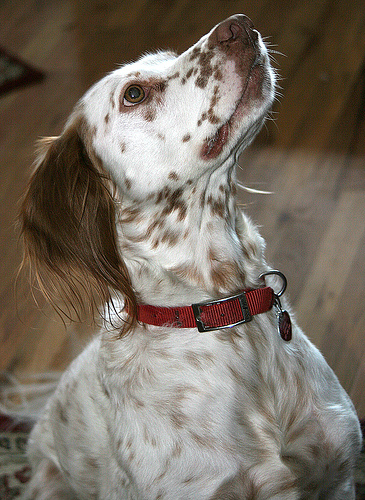
\includegraphics[width=\textwidth]{figures/task1/english_setter_178.jpg}
    \end{minipage}
    \begin{minipage}{0.28\textwidth}
        \centering
        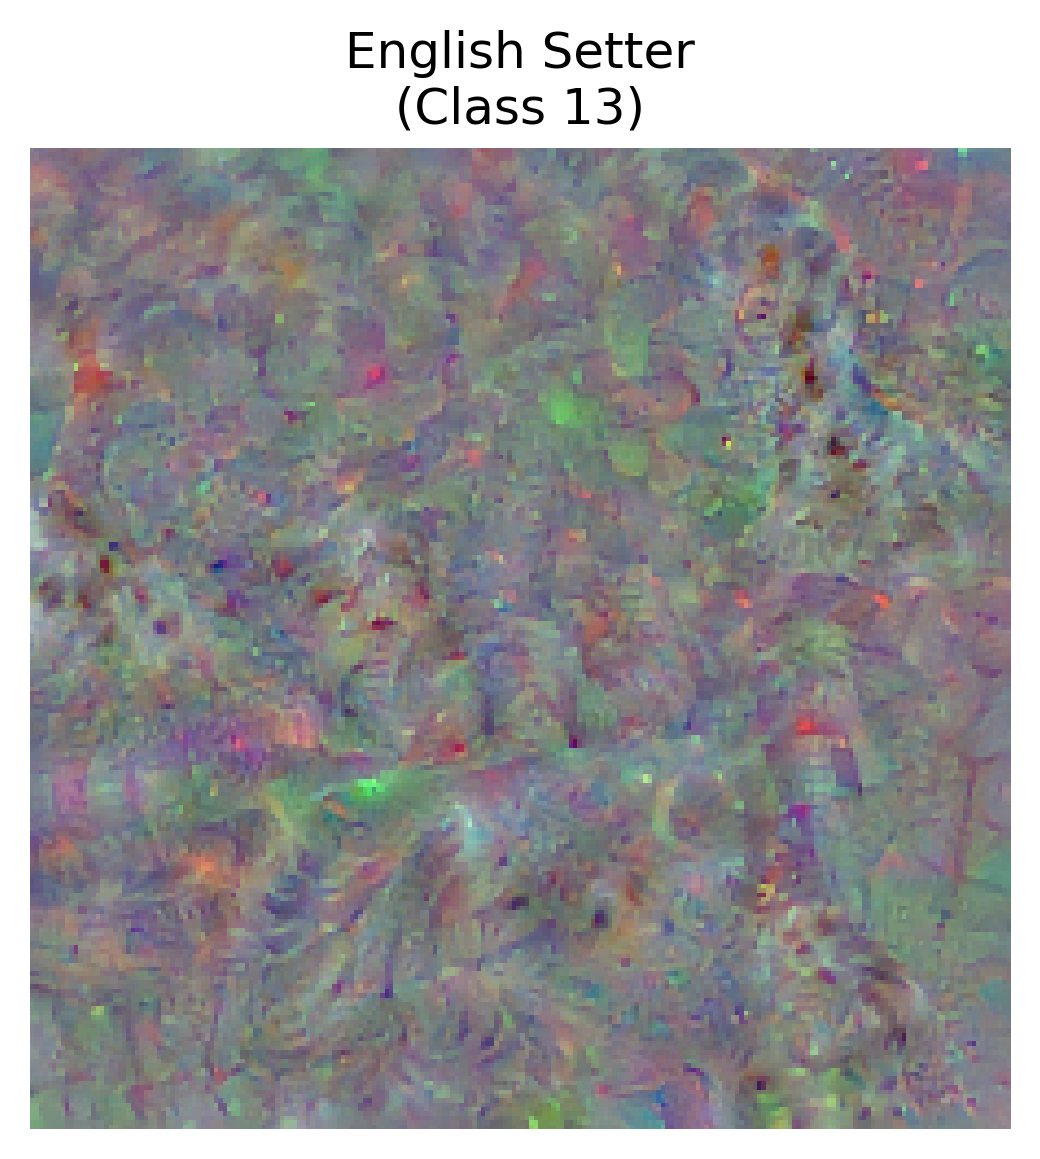
\includegraphics[width=\textwidth]{figures/task1/deep_dream_english_setter.png}
    \end{minipage}

    \vspace{0.5em}

    \begin{minipage}{0.24\textwidth}
        \centering
        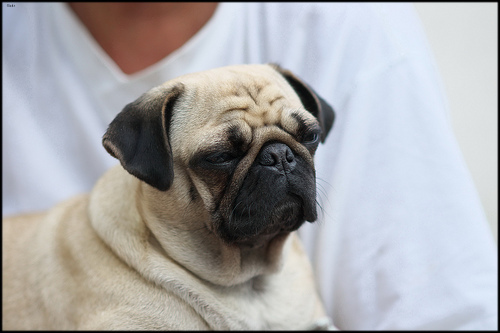
\includegraphics[width=\textwidth]{figures/task1/pug_85.jpg}
    \end{minipage}
    \begin{minipage}{0.28\textwidth}
        \centering
        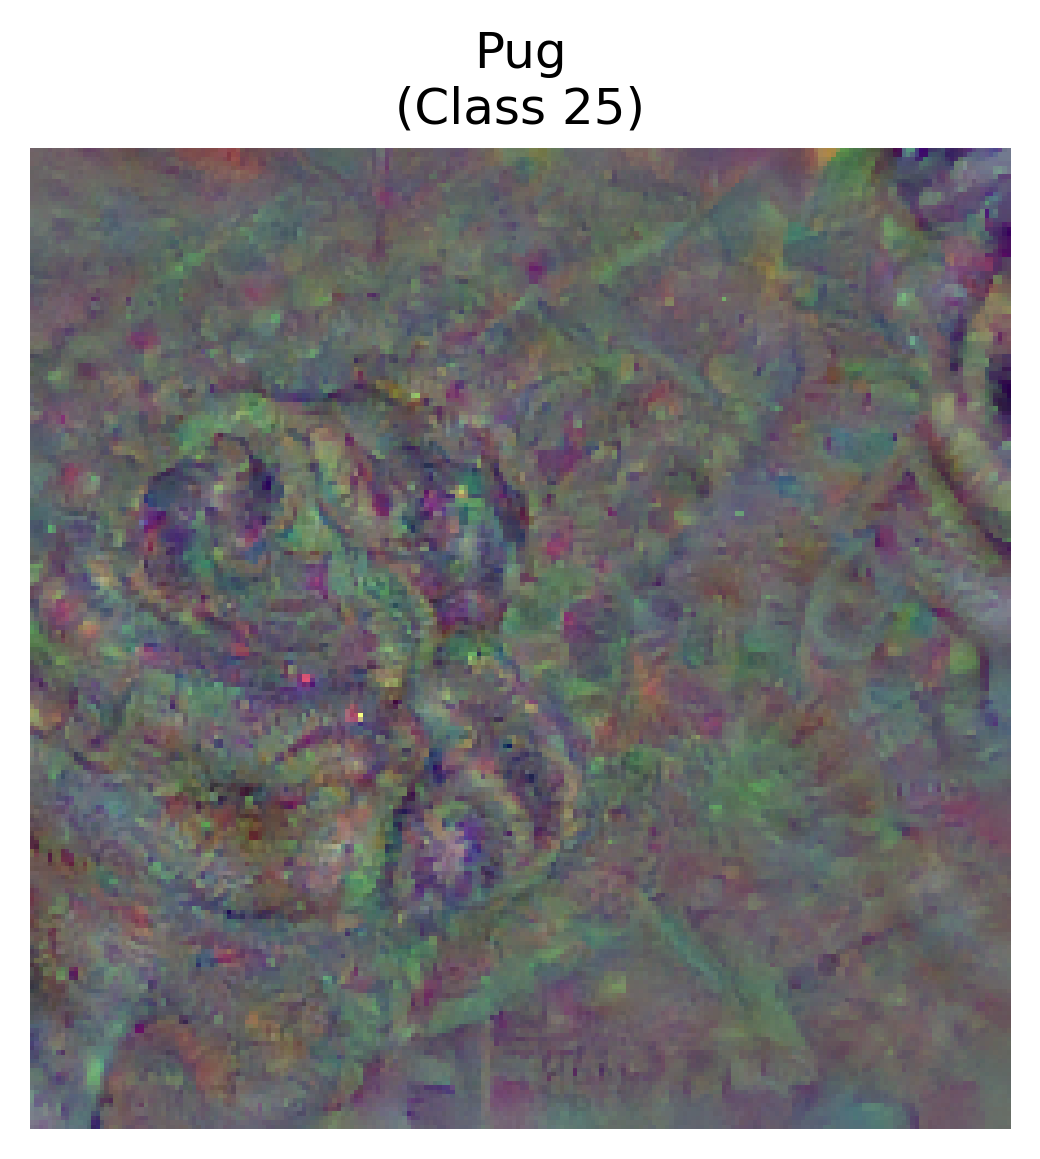
\includegraphics[width=\textwidth]{figures/task1/deep_dream_pug.png}
    \end{minipage}
    \hfill
    \begin{minipage}{0.15\textwidth}
        \centering
        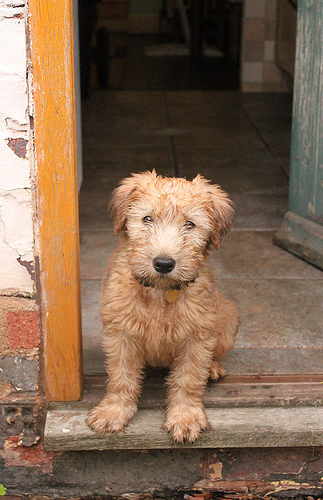
\includegraphics[width=\textwidth]{figures/task1/wheaten_terrier_43.jpg}
    \end{minipage}
    \begin{minipage}{0.28\textwidth}
        \centering
        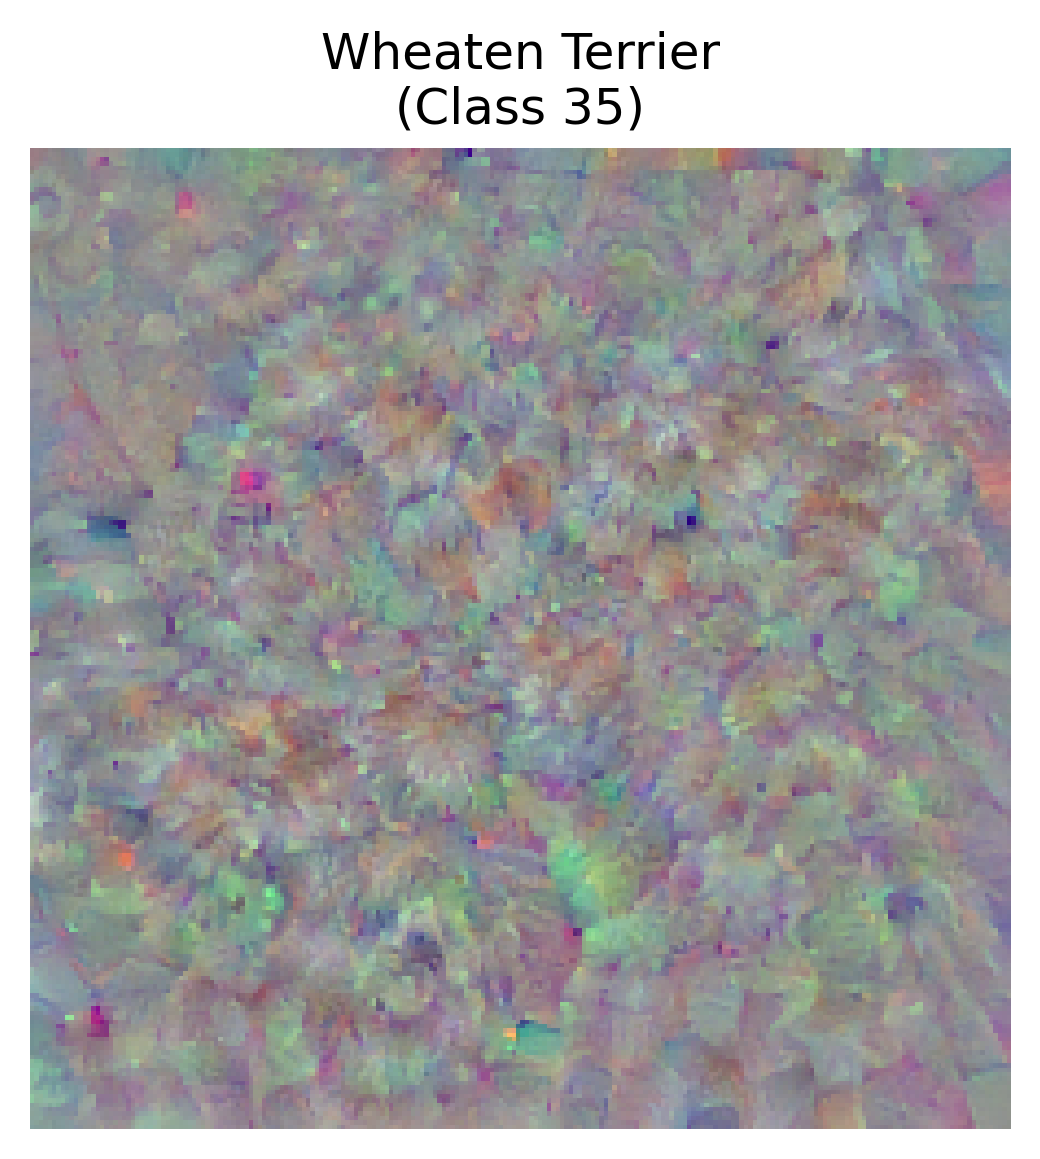
\includegraphics[width=\textwidth]{figures/task1/deep_dream_wheaten_terrier.png}
    \end{minipage}

    \caption{Representative images and DeepDream visualizations of their corresponding classes for four pet breeds. Top row: Basset Hound and English Setter. Bottom row: Pug and Wheaten Terrier.}
    \label{fig:deepdream_results}
\end{figure}

Several meaningful visual patterns can be observed. In the Basset Hound visualization, elongated ear-like structures and nose-like shapes emerge repeatedly, suggesting that the model captures distinctive shape information. In the English Setter visualization, spot-like textures become highly prominent, indicating sensitivity to fur pattern statistics. The Pug visualization contains dense folded textures resembling facial wrinkles, while the Wheaten Terrier visualization emphasizes fluffy fur-like structures.

These observations suggest that the network learns a combination of global shape cues and local texture patterns for fine-grained pet breed classification.
